\chapter{Llamadas a procedimientos remotos: GRPC}
\label{chap:grpc}

En mis objetivo planteo tener un componente en el servidor que administre y escale las funciones y una herramienta de línea de comandos para controlarlo todo. Quiero además que ese cliente use especificaciones que en un futuro puedan implementar otros clientes que innoven en algún aspecto siempre con la misma API por debajo. En este capítulo presentaré la tecnología que uso para comunicar el cliente y el servidor de forma segura, y que se podría usar en un futuro para comunicaciones internas del cluster igualmente.

GRPC es un framework RPC multilenguaje para la comunicación entre aplicaciones. Autogenera código en varios lenguajes para habilitar que se llame a métodos de forma sencilla que sin embargo tienen que cruzar la red para llegar al otro programa a ejecutarse.

Frameworks de este tipo existen muchos, especialmente en Java y otros lenguajes típicamente empresariales. GRPC difiere de ellos en que usa codificaciones y mecanismos de transporte altamente eficientes y que está implementado actualmente en producción para APIs de Google que reciben millones de peticiones sin parar.

\section{Protocol Buffers}
\label{sec:protobuf}

Para serializar los mensajes que se intercambian entre servidores se usa un lenguaje denominado \emph{Protocol Buffers}, acortado \emph{protobuf}. El lenguaje surgió en Google donde se usan varios lenguajes, principalmente Java, Go, Python y C++ para todos los servicios. Se buscaba un método de poder intercambiar y autogenerar los modelos para todos evitando errores de las copias manuales. Con la cantidad de datos que se manejan en los servidores se necesitaba una manera eficiente de leer y escribir esos modelos para mandarlos a otro servidor o guardarlos en disco.

Partiendo de un fichero en disco en un lenguaje propio se definen los mensajes y sus propiedades. Cada propiedad lleva un tipo asociado (cadena, número, otro mensaje, etc.) y un número identificador. Los números sirven para conservar la compatibilidad con versiones anteriores de nuestro protocolo aunque añadamos o renombremos propiedades.

Existen dos versiones de la sintaxis bastante parecidas. GRPC es compatible con la versión 3 (la última) que es la que usaré en todos los ejemplos y en mi aplicación.

Aquí tenemos un ejemplo que define dos mensajes (uno anidado) y una enumeración junto con las propiedades de cada mensaje:

\begin{minted}[baselinestretch=1.2]{protobuf}
message Person {
  string name = 1;
  int32 id = 2;
  string email = 3;

  enum PhoneType {
    MOBILE = 0;
    HOME = 1;
    WORK = 2;
  }

  message PhoneNumber {
    string number = 1;
    PhoneType type = 2 [default = HOME];
  }

  repeated PhoneNumber phone = 4;
}
\end{minted}

Un compilador lee el fichero y genera el código equivalente en el lenguaje elegido (Ruby, C\#, C++, Java, Python, Javascript, Go u otros). En cada versión mantiene las peculiaridades propias de la plataforma, como usar clases en Java o estructuras en Go.

En todos los lenguajes soportados hay métodos para escribir un modelo en una lista de bytes o leerlos a una nueva instancia. La escritura se realiza siguiendo una guía especificada\cite{protoencoding} que intenta obtener un formato binario eficiente y rápido para almacenar todo el abanico de tipos posibles. También existe una asociación directa a tipos de JSON\cite{protojson} para poder transformar a/desde ese formato.

Los protobufs se pueden usar en todo tipo de situaciones. Google por ejemplo lo usa para transferir los datos de Gmail al abrir la página (se pueden ver en el código fuente) o para escribir en disco los datos de su conocida y superescalable base de datos \emph{BigTable}\cite{bigtable}.

En GRPC se puede transferir un mensaje de petición (normalmente denominado \emph{FooRequest} para llamar a un método \emph{Foo}) y un mensaje de respuesta (\emph{FooReply} o \emph{FooResponse}). Éstos mensajes a su vez pueden contener otros anidados, así que las posibilidades son infinitas.

Existe un conjunto de tipos definidos en el mismo código fuente de protobuf denominados \emph{WellKnownTypes}\cite{wellknowntypes} que implementan las típicas necesidades de una comunicación, como un mensaje vacío, una fecha, una duración y otros. Podemos usar estos tipos para representar una llamada que no retorna respuesta por ejemplo, retornando un mensaje vacío y documentado para ese propósito como el de \emph{WellKnownTypes}, aunque no tenga ningún tratamiento especial por parte del compilador y aunque fuera similar a uno nuestro.

Para definir un servicio de GRPC se usa también sintaxis de protobuf:
\begin{minted}[baselinestretch=1.2]{protobuf}
service Dashboard {
    rpc Foo(FooRequest) returns (FooReply) {}
}

message FooRequest {
}

message FooReply {
}
\end{minted}

Al usar el compilador sobre un fichero protobuf con definiciones de servicios el plugin de GRPC genera código adicional en el mismo fichero para el cliente y el servidor de ese servicio.

\section{HTTP2}
\label{sec:http2}

Es de todos conocido la importancia que ha tenido HTTP para el desarrollo de cualquier comunicación web. Hasta ahora la versión más utilizada es la 1.1; que da vida a la mayor parte de las aplicaciones webs que visitamos. En 2015 se publicó una nueva versión en un RFC\cite{rfchttp2} después de varios años de trabajo adaptando una tecnología en pruebas de Google denominada \emph{SPDY}.

La nueva versión introdujo varias mejoras importantes con respecto a la anterior:
\begin{itemize}
    \item Las cabeceras de los mensajes se codificaban con un diccionario previo para comprimirlas.
    \item Se pueden enviar cabeceras tanto al principio como al final del contenido (\emph{trailers}).
    \item Se multiplexa la conexión para poder pedir o descargarse varios ficheros todo ello al mismo tiempo intercalando los paquetes de uno y otro.
    \item El servidor puede avisar al cliente de que se tiene que descargar varios ficheros juntos al mismo tiempo sin esperar a que lo descubra él. Esto se usa especialmente en webs para acelerar el tiempo de carga.
\end{itemize}

Con las recientes revelaciones de escuchas no autorizadas en masa por los servicios de inteligencia a servicios de internet claves como el correo electrónico casi cualquier nueva plataforma o protocolo sale siempre de una seguridad base más alta que antes. En este caso la mayor parte de los servidores, clientes, navegadores, etc. que entienden HTTP/2 lo hacen solamente cuando la conexión es segura (HTTPS).

GRPC usa HTTP como mecanismo para hacer llegar la petición y la respuesta entre las dos aplicaciones involucradas. Las direcciones URL se autogeneran siguen el nombre de los métodos que definamos en el fichero protobuf. Los servidores para escuchar nuevas conexiones y leerlas y los clientes para enviar datos se autogeneran también en todos los lenguajes según corresponda. La librería se encarga de gestionar las conexiones, los reintentos y otros temas de bajo nivel que no nos interesan al hacer la llamada al método.

La librería aprovecha las capacidades del protocolo para multiplexar conexiones con distintas llamadas, streams concurrentes de diferentes llamadas o incluso un stream bi-direccional entre el cliente y el servidor. Los \emph{trailers} se usan como mecanismo de transmisión de errores de vuelta al cliente una vez que la llamada ha concluido.

\section{Tipos de RPC}
\label{sec:rpc-types}

\subsection{RPC unarios}
\label{subsec:unary-rpc}

Los tipos más simples de RPC. Reciben un mensaje, emiten un mensaje y cierran la llamada inmediatamente.

Ejemplo con dos mensajes propios:
\begin{minted}[baselinestretch=1.2]{protobuf}
service Dashboard {
    rpc Foo(FooRequest) returns (FooReply) {}
}

message FooRequest {
}

message FooReply {
}
\end{minted}

Ejemplo con un mensaje vacío de \emph{WellKnownTypes}:
\begin{minted}[baselinestretch=1.2]{protobuf}
import "google/protobuf/empty.proto";

service Dashboard {
    rpc Foo(FooRequest) returns (google.protobuf.Empty) {}
}

message FooRequest {
}
\end{minted}

\subsection{RPC en streaming}
\label{subsec:streaming-rpc}

Las llamadas pueden devolver un stream continuo de datos que no termina el procedimiento hasta que deseemos cerrarlo nosotros. Podemos ir transmitiendo cada paquete de datos invidual y progresivamente en lugar de esperar a que esté todo listo.

\subsubsection{Hacia el servidor}
\label{subsubsec:in-streaming}

Permiten al cliente enviar la petición progresivamente al servidor. Ejemplo:
\begin{minted}[baselinestretch=1.2]{protobuf}
service Dashboard {
    rpc Foo(stream FooRequest) returns (FooReply) {}
}

message FooRequest {
}

message FooReply {
}
\end{minted}

\subsubsection{Desde el servidor}
\label{subsubsec:out-streaming}

Permiten al servidor enviar la respuesta progresivamente al cliente. Ejemplo:
\begin{minted}[baselinestretch=1.2]{protobuf}
service Dashboard {
    rpc Foo(FooRequest) returns (stream FooReply) {}
}

message FooRequest {
}

message FooReply {
}
\end{minted}

\subsubsection{Bidireccionales}
\label{subsubsec:bi-streaming}

Permiten que se hablen mutuamente el servidor y el cliente con una comunicación bidireccional. Ambos pueden escribir o leer en el orden que deseen, el servidor no tiene que esperar a recibir todos los datos para empezar a enviar respuesta y viceversa. Ejemplo:
\begin{minted}[baselinestretch=1.2]{protobuf}
service Dashboard {
    rpc Foo(stream FooRequest) returns (stream FooReply) {}
}

message FooRequest {
}

message FooReply {
}
\end{minted}

\subsection{RPC Mixtos}
\label{subsec:mixed-rpc}

Las llamadas son independientes entre sí, se pueden mezclar los distintos tipos de RPC en un mismo servicio sin ningún problema:

\begin{minted}[baselinestretch=1.2]{protobuf}
service Dashboard {
    rpc Foo(FooRequest) returns (FooReply) {}
    rpc Foo2(FooRequest) returns (stream FooReply) {}
    rpc Foo3(stream FooRequest) returns (stream FooReply) {}
}

message FooRequest {
}

message FooReply {
}
\end{minted}

\section{Seguridad}
\label{sec:grpc-security}

GRPC se aprovecha de la seguridad que nos puede dar el protocolo usando HTTPS para las conexiones. Algo que no es normal en un navegador web típico es usar certificados también para el cliente, pero si se pueden usar con este framework. Estos certificados nos dan varias ventajas:
\begin{itemize}
    \item Autenticación del servidor: sabemos que nos comunicamos con la máquina correcta de forma segura.
    \item Autenticación del cliente: sabemos que es un cliente autorizado para conectarse con nuestra máquina. Evitamos cualquier intento de ataque contra el servicio.
    \item Autorización del cliente: sabemos el cliente que es en concreto leyendo los datos del certificado y podemos determinar si está autorizado a ejecutar esa acción sobre el servicio o no.
\end{itemize}

Los certificados pueden ser autogenerados sin problemas, dado que es nuestro servicio y podemos usar esas claves generadas como las únicas autorizadas para usar el servicio. El propio cliente/servidor de GRPC se encarga de validar que la cadena de firmas corresponda a ese conjunto.

\section{Tracing de peticiones}
\label{sec:trace}

El framework en su versión de Go tiene configurado una librería trazadora de peticiones\cite{nettrace}, que registra métricas de rendimiento a lo largo de la vida del sistema y los datos que entran y salen de las últimas peticiones hechas.

Esta herramienta tan simple es de un valor incalculable cuando queremos depurar problemas y tenemos que determinar en qué servicio se ha empezado a cambiar los datos de una manera inesperada. Además genera un histograma bastante primitivo de los tiempos de respuesta que sirve para analizar peticiones que hayan tardado demasiado para lo que teníamos planeado.

El diseño está inspirado en la funcionalidad que Google usa internamente con Dapper\cite{36356}, aunque la versión libre en Go no puede trazar peticiones entre servicios, se limita a cada instancia individualmente.

Cuando entramos a la URL de la herramienta nos da un listado de métodos que está trazando como se ve en la figura \ref{fig:trace-dashboard}. Podemos obtener un histograma del último minuto, hora y en total, bastante primitivo como se observa en la figura \ref{fig:trace-histogram} pero bastante efectivo también. Por último para depurar podemos obtener los últimos mensajes intercambiados en cada cubo de tiempo que hay arriba, o el cubo de errores que está al final. Podemos simplemente listarlos como en la figura \ref{fig:trace-requests} o expandirlos para ver la información intercambiada y otros registros que hayamos dejado en los logs nosotros como en la figura \ref{fig:trace-expanded}.

\begin{figure}[H]
    \centering
    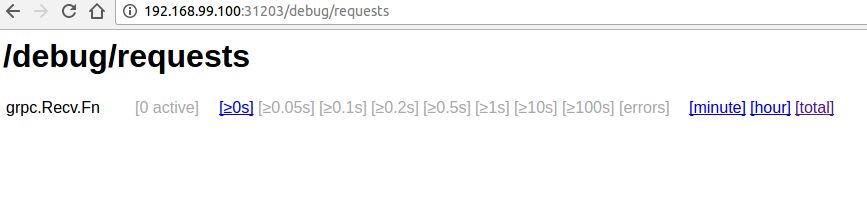
\includegraphics[width=\textwidth]{../images/trace/dashboard.png}
    \caption{Pantalla inicial para trazar}
    \label{fig:trace-dashboard}
\end{figure}

\begin{figure}[H]
    \centering
    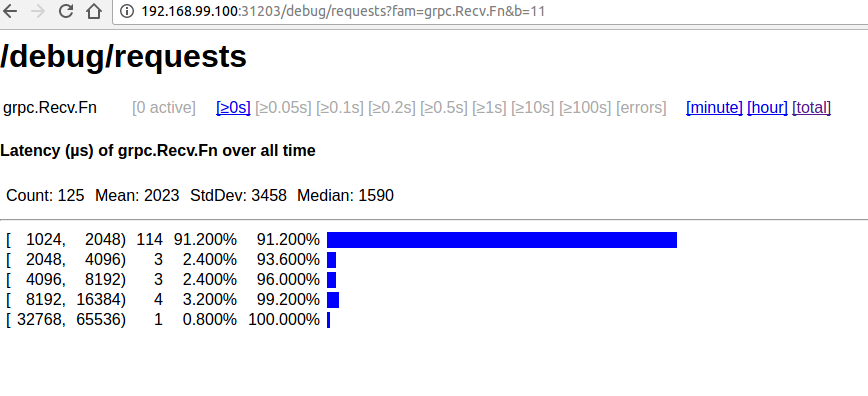
\includegraphics[width=\textwidth]{../images/trace/histogram.png}
    \caption{Histograma con los tiempos de respuesta desde que empezó el servidor}
    \label{fig:trace-histogram}
\end{figure}

\begin{figure}[H]
    \centering
    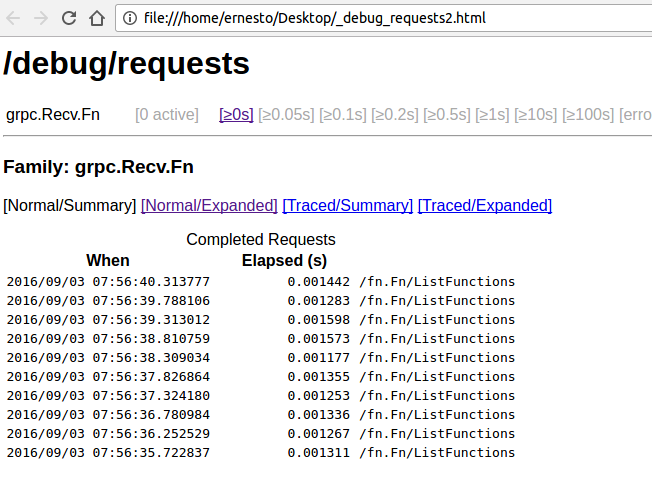
\includegraphics[width=\textwidth]{../images/trace/requests.png}
    \caption{Listado de peticiones del cubo de todas ellas (mayor a cero)}
    \label{fig:trace-requests}
\end{figure}

\begin{figure}[H]
    \centering
    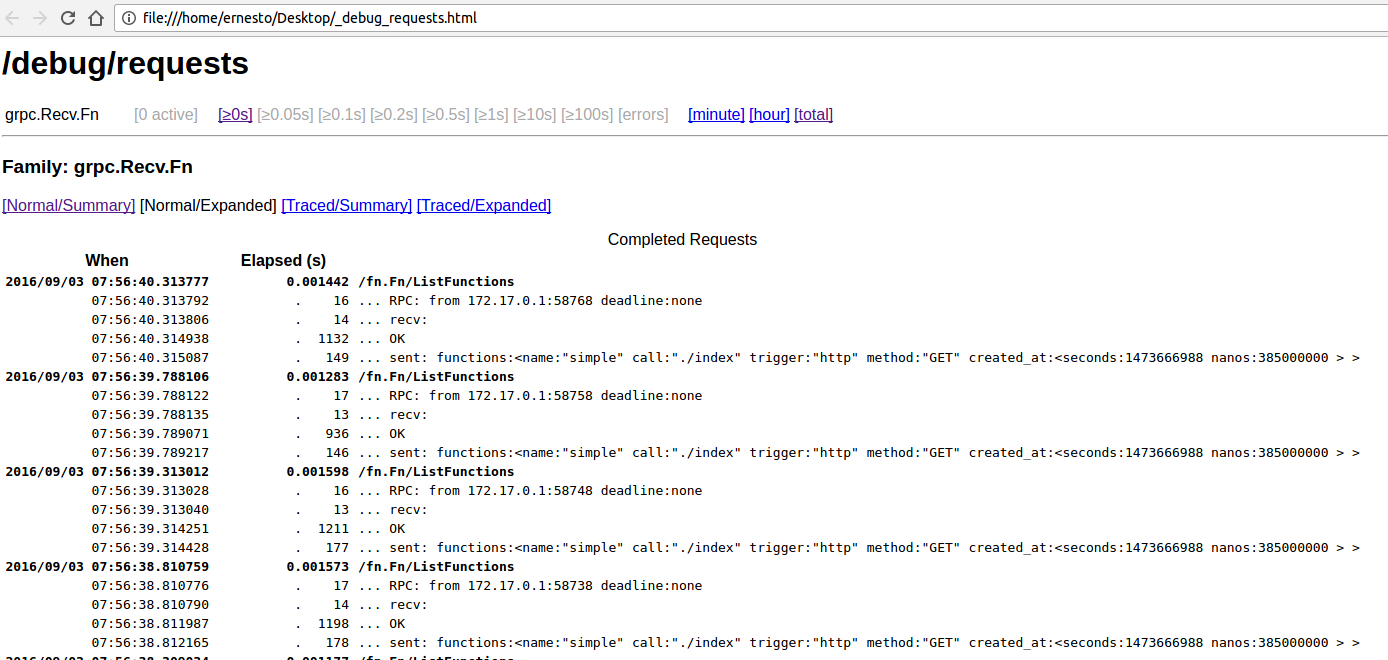
\includegraphics[width=\textwidth]{../images/trace/expanded.png}
    \caption{Listado de las últimas peticiones expandidas}
    \label{fig:trace-expanded}
\end{figure}

\section{Alternativas}
\label{sec:grpc-alternatives}

Realmente es difícil encontrar un framework que cubra todo el proceso de diseño desde los mensajes que se van a trasladar, pasando por la generación multilenguaje del código y llegando a la depuración y monitorización en producción. Aún más difícil si buscamos la estabilidad de años en servicios de producción bajo una carga reseñable.

\subsection{SOAP}
\label{subsec:alt-soap}

SOAP parte de una definición XML del intercambio de mensajes para generar el código. No lo he usado por varias razones:
\begin{itemize}
    \item Existen varios estándares según la herramienta que escojas y a veces es dificil usar todas las librerías en común.
    \item El formato de texto XML no es tan eficiente como el binario optimizado de Protobuf.
    \item GRPC genera servidores más eficientes usando los últimos avances de compresión y multiplexación de HTTP/2.
    \item GRPC tiene ya integradas cuestiones de seguridad usando certificados para evitar que nadie espíe ni corrompa la transmisión.
\end{itemize}

\subsection{REST}
\label{subsec:alt-rest}

REST más que un framework es una guía a seguir para exponer tus recursos en URLs de una forma ordenada y casi autodocumentada. Existen ciertos avances en la autogeneración de código como Swagger Codegen\cite{swaggercodegen} que aún así se quedan cortos a la hora de tener un servidor realmente optimizado y objetivamente listo para poner en producción tal cual.

GRPC define las operaciones como servicios y sus métodos, en lugar de recursos y operaciones sobre recursos; no he heredado prácticamente nada de REST en mi proyecto.

\subsection{Apache Thrift}
\label{subsec:thrift}

Thrift\cite{thrift} es seguramente el competidor que sigue más de cerca las características que ofrece GRPC. Genera servidores y clientes en varios lenguajes diferentes y usa un protocolo binario para transmitir los mensajes. El lenguaje para definir servicios y mensajes es parecido a Protobuf en muchos sentidos.

No la he usado porque:
\begin{itemize}
    \item Para mi gusto introduce detalles de bajo nivel, como tener que tener que usar explícitamente un buffer para los sockets, que no corresponden a un framework de estas características. La librería debería encargarse de configurar la red como necesite.
    \item No está excesivamente documentado. Apenas unas wikis y ejemplos dispersos incluso con errores por la antigüedad.
    \item Ha ido perdiendo impulso y el desarrollo parece estancado desde que Facebook dejó a su suerte el proyecto. Se crean muchas issues de errores que no tienen capacidad de solucionar como se ve por las estadísticas generales del proyecto\cite{thriftjira}.
\end{itemize}
